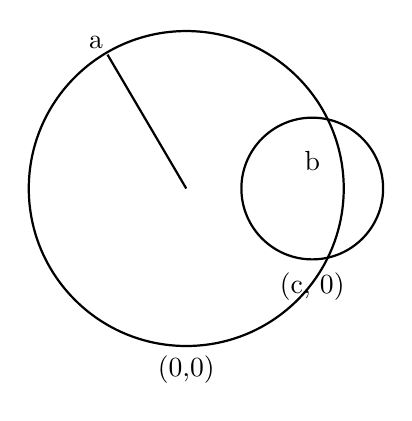
\begin{tikzpicture}[scale=1]
  % large circle centered at (0,0)
  \draw[thick] (0,0) circle (2.0);
  \node at (0,-2.3) {(0,0)};
  % small circle centered at (c,0), labeled b, radius drawn to upper-right
  \draw[thick] (1.6,0) circle (0.9);
  \node at (1.6,0.35) {b};
  \node at (1.6,-1.25) {(c, 0)};
  % radius line "a" from origin going up-left, outside both circles
  \draw[thick] (0,0) -- (-1.0,1.7);
  \node at (-1.15,1.85) {a};
\end{tikzpicture}
